\documentclass[answers]{exam}
\usepackage{texPreamble}
\usepackage{relsize}
\usepackage{tabularx}
\extraheadheight{0.25in}
\extrafootheight{1.0in}
\extrawidth{1in}
% ----------------------------------------------------------------

\begin{document}
%\relscale{1.4}
  \section{2.2: Definitions of Limits}
    \begin{defn*}(Briggs)
      Suppose the function $f$ is defined for all $x$ near $a$ except possibly at $a$. If $f(x)$ is arbitrarily close to $L$ (as close to $L$ as we like) for all $x$ sufficiently close (but not equal) to $a$, we write
        $$\lim_{x\to a} f(x)=L$$
      and say the limit of $f(x)$ as $x$ approaches $a$ equals $L$.
    \end{defn*}
    \textit{Note--} Most of the time, we can think of the limit as the value of the function if it could be evaluated at a specific point.
    \vspace*{\stretch{1}}
      
    \begin{ex*}
      Using the graph of $f$, determine the following values:\\[\stretch{1}]

      \noindent
      \begin{minipage}[b]{0.55\linewidth}
        \begin{itemize}
          \item $f(1)$ and $\ds\lim_{x\to 1}f(x)$\\[0.8in]
          \item $f(2)$ and $\ds\lim_{x\to 2}f(x)$\\[0.8in]
          \item $f(3)$ and $\ds\lim_{x\to 3}f(x)$\\[0.8in]
        \end{itemize}
      \end{minipage}%
      \begin{minipage}[b]{0.45\linewidth}
        \strut\vspace*{-\baselineskip}\newline
        \begin{flushright}
          \begin{tikzpicture}
            \begin{axis}[
              grid=both,
              grid style={line width=0.35pt, draw=gray!75},
              axis lines=center,
              axis line style={->},
              xmin=-1, xmax=6.5,
              ymin=-1, ymax=6.5,
              xtick={0,1,...,6},
              ytick={0,1,...,6},
              ticklabel style={fill=white},
              xlabel=$x$, xlabel style={at={(ticklabel* cs:1)},anchor=north west},
              ylabel=$f(x)$, ylabel style={at={(ticklabel* cs:1)},anchor=south west},
              every axis plot/.append style={line width=0.95pt}
              ]
              \addplot[<->] expression[domain=0:6.25, samples=250] {(x-2)/abs(x-2)*abs(x-2)^(1/3)+3};
              \addplot[holdot] coordinates{(2,3)(3,4)};
              \addplot[soldot] coordinates{(2,5)};
            \end{axis}
          \end{tikzpicture}
        \end{flushright}
      \end{minipage}
    \end{ex*}
    \pagebreak
      
      \begin{defn*}(Briggs)
        \begin{enumerate}
          \item \textbf{Right-sided limit} Suppose $f$ is defined for all $x$ near $a$ with $x>a$. If $f(x)$ is arbitrarily close to $L$ for all $x$ sufficiently close to $a$ with $x>a$, we write
            $$\lim_{x\to a^+}f(x)=L$$
          and say the limit of $f(x)$ as $x$ approaches $a$ from the right equals $L$.
          \item \textbf{Left-sided limit} Suppose $f$ is defined for all $x$ near $a$ with $x<a$. If $f(x)$ is arbitrarily close to $L$ for all $x$ sufficiently close to $a$ with $x<a$, we write
            $$\lim_{x\to a^-}f(x)=L$$
          and say the limit of $f(x)$ as $x$ approaches $a$ from the left equals $L$.
        \end{enumerate}
      \end{defn*}
      
      \vspace*{\stretch{1}}
      \noindent
        \begin{minipage}[b]{0.5\linewidth}
          \begin{ex*}
            For $f(x)=\dfrac{x^3-8}{4(x-2)}$, find
            \begin{itemize}
              \item $\ds\lim_{x\to2^+}f(x)$\\[0.95in]
              \item $\ds\lim_{x\to2^-}f(x)$\\[0.95in]
            \end{itemize}
          \end{ex*}
        \end{minipage}%
        \begin{minipage}[b]{0.5\linewidth}
        \strut\vspace*{-\baselineskip}\newline
          \begin{flushright}
            \begin{tikzpicture}
              \begin{axis}[
                axis lines=center,
                axis line style={->},
                xmin=-0.5, xmax=3.5,
                ymin=-0.6, ymax=4.5,
                xtick={0,1,...,3},
                ytick={0,1,...,8},
                ticklabel style={fill=white},
                xlabel=$x$, xlabel style={at={(ticklabel* cs:1)},anchor=north west},
                ylabel=$f(x)$, ylabel style={at={(ticklabel* cs:1)},anchor=south west},
                every axis plot/.append style={line width=0.95pt}
              ]
              \addplot[<->] expression[domain=-0.5:2.75] {(x^2+2*x+4)/4};
              \addplot[holdot] coordinates{(2,3)};
              \end{axis}
            \end{tikzpicture}
          \end{flushright}
        \end{minipage}%
      
      \pagebreak
      
      \begin{defn*}(Briggs)
        \textbf{Relationship Between One-Sided and Two-Sided Limits}
        
        Assume $f$ is defined for all $x$ near $a$ except possibly at $a$. Then $\ds\lim_{x\to a}f(x)=L$ if and only if $\ds\lim_{x\to a^+}f(x)=L$ and $\ds\lim_{x\to a^-} f(x)=L$. 
      \end{defn*}
      \begin{ex*}
        For $f(x)$ above, is $\ds\lim_{x\to2}f(x)$ defined? If so, what is it? What is $f(2)$?
      \end{ex*}
      \vspace*{\stretch{1}}
      \noindent 
      \begin{minipage}[b]{0.55\linewidth}
        \begin{ex*}
          Consider the graph of 
          \begin{align*}
            g(x)&=\dfrac{2x^2-6x+4}{\abs{x-1}}
              =\begin{cases}
              -2(x-2)& x<1\\
              2(x-2)& x>1
            \end{cases}
          \end{align*}
          Find
          \begin{itemize}
            \item $\ds\lim_{x\to1^-}g(x)$\\[0.5in]
            \item $\ds\lim_{x\to1^+}g(x)$\\[0.5in]
            \item $\ds\lim_{x\to1}g(x)$\\[0.5in]
          \end{itemize}
        \end{ex*}
      \end{minipage}%
      \begin{minipage}[b]{0.45\linewidth}
      \strut\vspace*{-\baselineskip}\newline
        \begin{flushright}
          \begin{tikzpicture}
            \begin{axis}[
              axis lines=center,
              axis line style={->},
              xmin=-0.5, xmax=3.5,
              ymin=-2.5, ymax=4.5,
              xtick={0,1,...,3},
              ytick={-2,-1,...,4},
              ticklabel style={fill=white},
              xlabel=$x$, xlabel style={at={(ticklabel* cs:1)},anchor=north west},
              ylabel=$g(x)$, ylabel style={at={(ticklabel* cs:1)},anchor=south west},
              every axis plot/.append style={line width=0.95pt}
              ]
              \addplot[<-] expression[domain=-0.25:1, blue] {-2*(x-2)};
              \addplot[->] expression[domain=1:3.25, blue] {2*(x-2)};
              \addplot[holdot] coordinates{(1,2)(1,-2)};
            \end{axis}
          \end{tikzpicture}
        \end{flushright}
      \end{minipage}
      \pagebreak
      
      \begin{ex*}
        Consider the function
          $$h(x)=\frac{x^2-81}{2x+18}$$
        What does this function look like? What is $h(-9)$? What is $\ds\lim_{x\to-9} h(x)$?
      \end{ex*}
      \vspace*{\stretch{1}}
      \noindent 
      \begin{minipage}[t]{0.6\linewidth}\ 
        \begin{ex*}
          The ceiling function is 
            $$j(x)=\ceil{x}$$
          where $\ceil{x}$ returns the smallest integer greater than or equal to $x$. In other words, the ceiling function always rounds up. Find the following: %(What do you think the floor function does?)
        \end{ex*}
      \end{minipage}%
      \begin{minipage}[t]{0.4\linewidth}\ 
        \begin{flushright}
          \begin{tikzpicture}
            \begin{axis}[
              axis equal,
              axis lines=center,
              axis line style={->},
              xmin=-2.25, xmax=3.25,
              ymin=-2.25, ymax=3.25,
              xtick={-3,-2,...,3},
              ytick={-2,-1,...,4},
              ticklabel style={fill=white},
              every axis plot/.append style={line width=0.95pt}
              ]
              \addplot[blue, domain=-2.5:3, jump mark mid] {ceil(x)};
              \addplot[holdot] coordinates{(-2,-1)(-1,0)(0,1)(1,2)(2,3)};
              \addplot[soldot] coordinates{(-2,-2)(-1,-1)(0,0)(1,1)(2,2)(3,3)};
            \end{axis}
          \end{tikzpicture}
        \end{flushright}
      \end{minipage}
      \begin{minipage}{11.5pt}
        \ 
      \end{minipage}%
      \vspace*{\stretch{0.1}}
      \begin{tasks}[after-item-skip=0.5\baselineskip, label=](4)
        \task[] $\ds\lim_{x\to 1^-} j(x)$ 
        \task[] $\ds\lim_{x\to 1^+} j(x)$ 
        \task[] $\ds\lim_{x\to 1} j(x)$ 
        \task[] $j(1)$
        \task[] $\ds\lim_{x\to 1.5^-} j(x)$ 
        \task[] $\ds\lim_{x\to 1.5^+} j(x)$ 
        \task[] $\ds\lim_{x\to 1.5} j(x)$ 
        \task[] $j(1.5)$ 
      \end{tasks}
      \vspace*{\stretch{0.1}}
      \pagebreak
      \begin{ex*}
        Consider the function
          $$h(x)=\cos\parens{\frac{1}{x}}$$
        What is $\ds\lim_{x\to0} h(x)$?
        
        \begin{minipage}{0.6\linewidth}
          Consider $x=1/(n\pi)$. As $n\to\infty, x\to0$, then,
            $$\cos\parens{\frac{1}{x}}=\cos\parens{n\pi}=
            \begin{cases}
              1& \text{if } n\text{ is even}\\
              -1& \text{if } n\text{ is odd}
            \end{cases}$$
        \end{minipage}%
        \begin{minipage}{0.4\linewidth}
          \begin{flushright}
            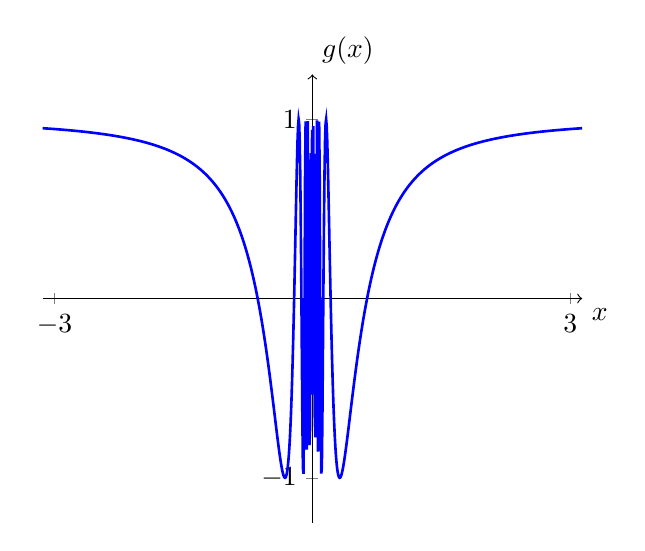
\begin{tikzpicture}
              \begin{axis}[
                axis lines=center,
                axis line style={->},
                xmin=-3.14, xmax=3.14,
                ymin=-1.25, ymax=1.25,
                xtick={-3,3},
                ytick={-1,1},
                ticklabel style={fill=white},
                xlabel=$x$, xlabel style={at={(ticklabel* cs:1)},anchor=north west},
                ylabel=$g(x)$, ylabel style={at={(ticklabel* cs:1)},anchor=south west},                every axis plot/.append style={line width=0.95pt}
                ]
              \addplot[-] expression[domain=-3.14:3.14, samples=1000, blue] {cos(deg 1/x)};
              \end{axis}
            \end{tikzpicture}
          \end{flushright}
        \end{minipage}
      \end{ex*}
      \vspace*{\stretch{1}}
      \begin{ex*}
        Graph an example with the following characteristics:
          $$\lim_{x\to-2^-} f(x)=-4\qquad 
            \lim_{x\to-2^+} f(x)= 2\qquad
            f(-2)=0\qquad$$
          $$\lim_{x\to4} f(x) = 2\qquad
            f(4) \textbf{ DNE}$$
          $$\lim_{x\to8} f(x) =-2\qquad
            f(8)=-2
            $$
        \begin{center}
          \begin{tikzpicture}
            \begin{axis}[
              axis lines=center,
              axis line style={->},
              height=2in, width=8in,
              xmin=-10, xmax=10,
              ymin=-6, ymax=6,
              xtick={-10,-8,...,10},
              ytick={-5,5},
              ticklabel style={fill=white},
              enlargelimits={abs=0.75},
              ]
            \end{axis}
          \end{tikzpicture}
        \end{center}
      \end{ex*}
      \pagebreak
\end{document}
